% Generated by recon/fig-method2.mjs --- do not edit by hand.
% Regenerate after any change to domain / grove-core / grove-objective.
\documentclass[tikz,border=2pt]{standalone}
\usepackage{amsmath,amssymb}
\usetikzlibrary{arrows.meta,patterns,decorations.pathreplacing}
\newcommand{\Feas}{\mathrm{Feasible}}
\definecolor{banditcol}{HTML}{2A78D6}
\definecolor{wifecol}{HTML}{EB6834}
\definecolor{samuraicol}{HTML}{1BAF7A}
\definecolor{inkcol}{HTML}{0B0B0B}
\definecolor{okcol}{HTML}{1B7A4A}
\definecolor{nocol}{HTML}{B03A2E}
\begin{document}
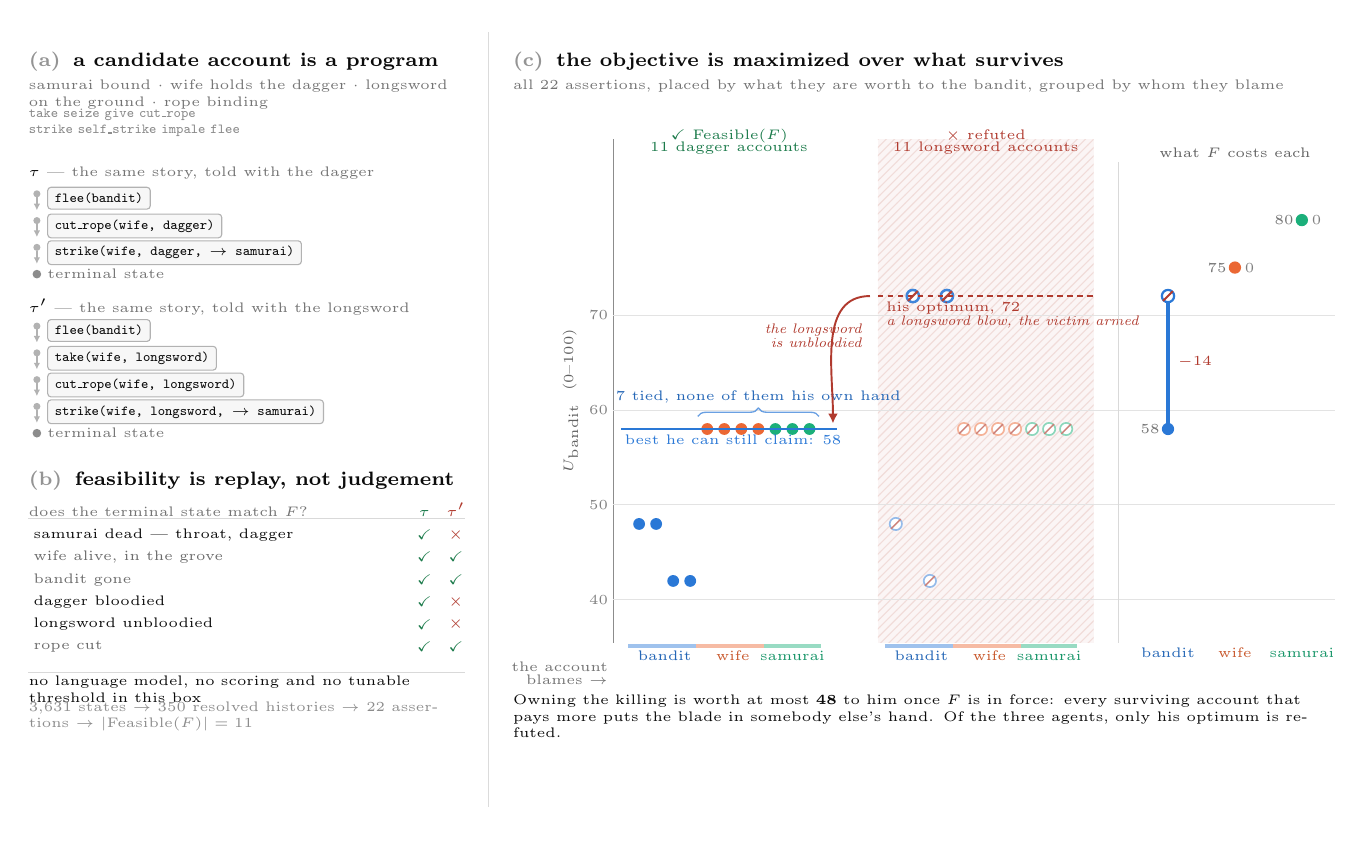
\begin{tikzpicture}[font=\small, inner sep=0pt]
  \path (0,0.30) rectangle (16.6,-9.7);
  \draw[gray!28, line width=0.4pt] (5.8500000000000005,0.24) -- (5.8500000000000005,-9.6);

  \node[anchor=north west, font=\scriptsize\bfseries, text=inkcol, align=left, text width=5.55cm] at (0,0) {\textcolor{black!42}{(a)}\, a candidate account is a program};
  \node[anchor=north west, font=\tiny, text=black!55, align=left, text width=5.55cm] at (0,-0.36) {samurai bound $\cdot$ wife holds the dagger $\cdot$ longsword on the ground $\cdot$ rope binding};
  \node[anchor=north west, font=\tiny\ttfamily, text=black!45, align=left, text width=5.55cm] at (0,-0.72) {take~seize~give~cut\_rope\\strike~self\_strike~impale~flee};
  \node[anchor=north west, font=\tiny, text=inkcol] at (0,-1.46) {$\tau$ \textcolor{black!55}{--- the same story, told with the dagger}};
  \fill[black!30] (0.11,-1.81) circle (0.045);
  \draw[-{Latex[length=2.4pt,width=2.4pt]}, black!30, line width=0.5pt] (0.11,-1.85) -- (0.11,-2.02);
  \node[anchor=north west, draw=black!30, line width=0.4pt, rounded corners=1.2pt, fill=black!3, inner xsep=2.6pt, inner ysep=2.0pt, font=\tiny\ttfamily, text=inkcol] at (0.24,-1.72) {flee(bandit)};
  \fill[black!30] (0.11,-2.15) circle (0.045);
  \draw[-{Latex[length=2.4pt,width=2.4pt]}, black!30, line width=0.5pt] (0.11,-2.19) -- (0.11,-2.36);
  \node[anchor=north west, draw=black!30, line width=0.4pt, rounded corners=1.2pt, fill=black!3, inner xsep=2.6pt, inner ysep=2.0pt, font=\tiny\ttfamily, text=inkcol] at (0.24,-2.06) {cut\_rope(wife, dagger)};
  \fill[black!30] (0.11,-2.4899999999999998) circle (0.045);
  \draw[-{Latex[length=2.4pt,width=2.4pt]}, black!30, line width=0.5pt] (0.11,-2.53) -- (0.11,-2.6999999999999997);
  \node[anchor=north west, draw=black!30, line width=0.4pt, rounded corners=1.2pt, fill=black!3, inner xsep=2.6pt, inner ysep=2.0pt, font=\tiny\ttfamily, text=inkcol] at (0.24,-2.4) {strike(wife, dagger, $\to$ samurai)};
  \fill[black!45] (0.11,-2.8299999999999996) circle (0.055);
  \node[anchor=west, font=\tiny, text=black!55] at (0.24,-2.8299999999999996) {terminal state};
  \node[anchor=north west, font=\tiny, text=inkcol] at (0,-3.1399999999999997) {$\tau'$ \textcolor{black!55}{--- the same story, told with the longsword}};
  \fill[black!30] (0.11,-3.4899999999999993) circle (0.045);
  \draw[-{Latex[length=2.4pt,width=2.4pt]}, black!30, line width=0.5pt] (0.11,-3.5299999999999994) -- (0.11,-3.6999999999999993);
  \node[anchor=north west, draw=black!30, line width=0.4pt, rounded corners=1.2pt, fill=black!3, inner xsep=2.6pt, inner ysep=2.0pt, font=\tiny\ttfamily, text=inkcol] at (0.24,-3.3999999999999995) {flee(bandit)};
  \fill[black!30] (0.11,-3.829999999999999) circle (0.045);
  \draw[-{Latex[length=2.4pt,width=2.4pt]}, black!30, line width=0.5pt] (0.11,-3.869999999999999) -- (0.11,-4.039999999999999);
  \node[anchor=north west, draw=black!30, line width=0.4pt, rounded corners=1.2pt, fill=black!3, inner xsep=2.6pt, inner ysep=2.0pt, font=\tiny\ttfamily, text=inkcol] at (0.24,-3.7399999999999993) {take(wife, longsword)};
  \fill[black!30] (0.11,-4.169999999999999) circle (0.045);
  \draw[-{Latex[length=2.4pt,width=2.4pt]}, black!30, line width=0.5pt] (0.11,-4.209999999999999) -- (0.11,-4.379999999999999);
  \node[anchor=north west, draw=black!30, line width=0.4pt, rounded corners=1.2pt, fill=black!3, inner xsep=2.6pt, inner ysep=2.0pt, font=\tiny\ttfamily, text=inkcol] at (0.24,-4.079999999999999) {cut\_rope(wife, longsword)};
  \fill[black!30] (0.11,-4.509999999999999) circle (0.045);
  \draw[-{Latex[length=2.4pt,width=2.4pt]}, black!30, line width=0.5pt] (0.11,-4.549999999999999) -- (0.11,-4.719999999999999);
  \node[anchor=north west, draw=black!30, line width=0.4pt, rounded corners=1.2pt, fill=black!3, inner xsep=2.6pt, inner ysep=2.0pt, font=\tiny\ttfamily, text=inkcol] at (0.24,-4.419999999999999) {strike(wife, longsword, $\to$ samurai)};
  \fill[black!45] (0.11,-4.849999999999999) circle (0.055);
  \node[anchor=west, font=\tiny, text=black!55] at (0.24,-4.849999999999999) {terminal state};
  \node[anchor=north west, font=\scriptsize\bfseries, text=inkcol, align=left, text width=5.55cm] at (0,-5.32) {\textcolor{black!42}{(b)}\, feasibility is replay, not judgement};
  \node[anchor=south, font=\tiny, text=okcol] at (5.029999999999999,-5.91) {$\tau$};
  \node[anchor=south, font=\tiny, text=nocol] at (5.43,-5.91) {$\tau'$};
  \node[anchor=south west, font=\tiny, text=black!55] at (0,-5.91) {does the terminal state match $F$?};
  \draw[gray!30, line width=0.4pt] (0,-5.930000000000001) -- (5.55,-5.930000000000001);
  \node[anchor=west, font=\tiny, text=inkcol] at (0.06,-6.140000000000001) {samurai dead --- throat, dagger};
  \node[font=\tiny, text=okcol] at (5.029999999999999,-6.140000000000001) {$\checkmark$};
  \node[font=\tiny, text=nocol] at (5.43,-6.140000000000001) {$\times$};
  \node[anchor=west, font=\tiny, text=black!58] at (0.06,-6.425000000000001) {wife alive, in the grove};
  \node[font=\tiny, text=okcol] at (5.029999999999999,-6.425000000000001) {$\checkmark$};
  \node[font=\tiny, text=okcol] at (5.43,-6.425000000000001) {$\checkmark$};
  \node[anchor=west, font=\tiny, text=black!58] at (0.06,-6.710000000000001) {bandit gone};
  \node[font=\tiny, text=okcol] at (5.029999999999999,-6.710000000000001) {$\checkmark$};
  \node[font=\tiny, text=okcol] at (5.43,-6.710000000000001) {$\checkmark$};
  \node[anchor=west, font=\tiny, text=inkcol] at (0.06,-6.995000000000001) {dagger bloodied};
  \node[font=\tiny, text=okcol] at (5.029999999999999,-6.995000000000001) {$\checkmark$};
  \node[font=\tiny, text=nocol] at (5.43,-6.995000000000001) {$\times$};
  \node[anchor=west, font=\tiny, text=inkcol] at (0.06,-7.280000000000001) {longsword unbloodied};
  \node[font=\tiny, text=okcol] at (5.029999999999999,-7.280000000000001) {$\checkmark$};
  \node[font=\tiny, text=nocol] at (5.43,-7.280000000000001) {$\times$};
  \node[anchor=west, font=\tiny, text=black!58] at (0.06,-7.565000000000001) {rope cut};
  \node[font=\tiny, text=okcol] at (5.029999999999999,-7.565000000000001) {$\checkmark$};
  \node[font=\tiny, text=okcol] at (5.43,-7.565000000000001) {$\checkmark$};
  \draw[gray!30, line width=0.4pt] (0,-7.8900000000000015) -- (5.55,-7.8900000000000015);
  \node[anchor=north west, font=\tiny, text=inkcol, align=left, text width=5.55cm] at (0,-7.9300000000000015) {no language model, no scoring and no tunable threshold in this box};
  \node[anchor=north west, font=\tiny, text=black!45, align=left, text width=5.55cm] at (0,-8.250000000000002) {3,631 states $\to$ 350 resolved histories $\to$ 22 assertions $\to$ $|\Feas(F)|=11$};
  \node[anchor=north west, font=\scriptsize\bfseries, text=inkcol, align=left, text width=10.450000000000001cm] at (6.15,0) {\textcolor{black!42}{(c)}\, the objective is maximized over what survives};
  \node[anchor=north west, font=\tiny, text=black!55, align=left, text width=10.450000000000001cm] at (6.15,-0.36) {all 22 assertions, placed by what they are worth to the bandit, grouped by whom they blame};
  \fill[nocol!5] (10.790000000000003,-7.51) rectangle (13.530000000000005,-1.1199999999999999);
  \fill[pattern=north east lines, pattern color=nocol!18] (10.790000000000003,-7.51) rectangle (13.530000000000005,-1.1199999999999999);
  \draw[black!45, line width=0.5pt] (7.430000000000001,-7.51) -- (7.430000000000001,-1.1199999999999999);
  \draw[gray!22, line width=0.35pt] (7.430000000000001,-6.9676) -- (16.6,-6.9676);
  \node[anchor=east, font=\tiny, text=black!50] at (7.370000000000001,-6.9676) {40};
  \draw[gray!22, line width=0.35pt] (7.430000000000001,-5.7616) -- (16.6,-5.7616);
  \node[anchor=east, font=\tiny, text=black!50] at (7.370000000000001,-5.7616) {50};
  \draw[gray!22, line width=0.35pt] (7.430000000000001,-4.5556) -- (16.6,-4.5556);
  \node[anchor=east, font=\tiny, text=black!50] at (7.370000000000001,-4.5556) {60};
  \draw[gray!22, line width=0.35pt] (7.430000000000001,-3.3495999999999997) -- (16.6,-3.3495999999999997);
  \node[anchor=east, font=\tiny, text=black!50] at (7.370000000000001,-3.3495999999999997) {70};
  \node[rotate=90, anchor=south, font=\tiny, text=black!62] at (6.99,-4.4350000000000005) {$U_{\mathrm{bandit}}$ \ (0--100)};
  \node[anchor=north east, font=\tiny, text=black!55, align=right] at (7.370000000000001,-7.75) {the account\\[-1.5pt]blames $\rightarrow$};
  \node[anchor=south, font=\tiny, align=center, text=okcol] at (8.9,-1.3199999999999998) {$\checkmark$ $\Feas(F)$\\[-1.5pt]11 dagger accounts};
  \draw[banditcol!45, line width=1.4pt] (7.618181818181819,-7.55) -- (8.547272727272729,-7.55);
  \node[anchor=north, font=\tiny, text=black!62, align=center] at (8.082727272727274,-7.61) {\color{banditcol!85!black}bandit};
  \draw[wifecol!45, line width=1.4pt] (8.483636363636364,-7.55) -- (9.412727272727274,-7.55);
  \node[anchor=north, font=\tiny, text=black!62, align=center] at (8.94818181818182,-7.61) {\color{wifecol!85!black}wife};
  \draw[samuraicol!45, line width=1.4pt] (9.34909090909091,-7.55) -- (10.061818181818184,-7.55);
  \node[anchor=north, font=\tiny, text=black!62, align=center] at (9.705454545454547,-7.61) {\color{samuraicol!85!black}samurai};
  \fill[banditcol] (7.758181818181819,-6.002800000000001) circle (0.075);
  \fill[banditcol] (7.9745454545454555,-6.002800000000001) circle (0.075);
  \fill[banditcol] (8.190909090909091,-6.7264) circle (0.075);
  \fill[banditcol] (8.407272727272728,-6.7264) circle (0.075);
  \fill[wifecol] (8.623636363636365,-4.7968) circle (0.075);
  \fill[wifecol] (8.840000000000002,-4.7968) circle (0.075);
  \fill[wifecol] (9.056363636363638,-4.7968) circle (0.075);
  \fill[wifecol] (9.272727272727273,-4.7968) circle (0.075);
  \fill[samuraicol] (9.48909090909091,-4.7968) circle (0.075);
  \fill[samuraicol] (9.705454545454547,-4.7968) circle (0.075);
  \fill[samuraicol] (9.921818181818184,-4.7968) circle (0.075);
  \node[anchor=south, font=\tiny, align=center, text=nocol] at (12.160000000000004,-1.3199999999999998) {$\times$ refuted\\[-1.5pt]11 longsword accounts};
  \draw[banditcol!45, line width=1.4pt] (10.878181818181819,-7.55) -- (11.80727272727273,-7.55);
  \node[anchor=north, font=\tiny, text=black!62, align=center] at (11.342727272727274,-7.61) {\color{banditcol!85!black}bandit};
  \draw[wifecol!45, line width=1.4pt] (11.743636363636366,-7.55) -- (12.672727272727276,-7.55);
  \node[anchor=north, font=\tiny, text=black!62, align=center] at (12.20818181818182,-7.61) {\color{wifecol!85!black}wife};
  \draw[samuraicol!45, line width=1.4pt] (12.609090909090911,-7.55) -- (13.321818181818186,-7.55);
  \node[anchor=north, font=\tiny, text=black!62, align=center] at (12.965454545454548,-7.61) {\color{samuraicol!85!black}samurai};
  \fill[white] (11.01818181818182,-6.002800000000001) circle (0.078);
  \draw[banditcol!50, line width=0.6pt] (11.01818181818182,-6.002800000000001) circle (0.078);
  \draw[nocol!65, line width=0.5pt] (10.95618181818182,-6.064800000000001) -- (11.080181818181819,-5.9408);
  \fill[white] (11.234545454545456,-3.1084000000000005) circle (0.078);
  \draw[banditcol!90, line width=0.9pt] (11.234545454545456,-3.1084000000000005) circle (0.078);
  \draw[nocol!95, line width=0.8pt] (11.172545454545457,-3.1704000000000003) -- (11.296545454545456,-3.0464000000000007);
  \fill[white] (11.450909090909093,-6.7264) circle (0.078);
  \draw[banditcol!50, line width=0.6pt] (11.450909090909093,-6.7264) circle (0.078);
  \draw[nocol!65, line width=0.5pt] (11.388909090909094,-6.7884) -- (11.512909090909092,-6.6644);
  \fill[white] (11.66727272727273,-3.1084000000000005) circle (0.078);
  \draw[banditcol!90, line width=0.9pt] (11.66727272727273,-3.1084000000000005) circle (0.078);
  \draw[nocol!95, line width=0.8pt] (11.60527272727273,-3.1704000000000003) -- (11.729272727272729,-3.0464000000000007);
  \fill[white] (11.883636363636366,-4.7968) circle (0.078);
  \draw[wifecol!50, line width=0.6pt] (11.883636363636366,-4.7968) circle (0.078);
  \draw[nocol!65, line width=0.5pt] (11.821636363636367,-4.8588000000000005) -- (11.945636363636366,-4.7348);
  \fill[white] (12.100000000000003,-4.7968) circle (0.078);
  \draw[wifecol!50, line width=0.6pt] (12.100000000000003,-4.7968) circle (0.078);
  \draw[nocol!65, line width=0.5pt] (12.038000000000004,-4.8588000000000005) -- (12.162000000000003,-4.7348);
  \fill[white] (12.31636363636364,-4.7968) circle (0.078);
  \draw[wifecol!50, line width=0.6pt] (12.31636363636364,-4.7968) circle (0.078);
  \draw[nocol!65, line width=0.5pt] (12.25436363636364,-4.8588000000000005) -- (12.37836363636364,-4.7348);
  \fill[white] (12.532727272727275,-4.7968) circle (0.078);
  \draw[wifecol!50, line width=0.6pt] (12.532727272727275,-4.7968) circle (0.078);
  \draw[nocol!65, line width=0.5pt] (12.470727272727276,-4.8588000000000005) -- (12.594727272727274,-4.7348);
  \fill[white] (12.749090909090912,-4.7968) circle (0.078);
  \draw[samuraicol!50, line width=0.6pt] (12.749090909090912,-4.7968) circle (0.078);
  \draw[nocol!65, line width=0.5pt] (12.687090909090912,-4.8588000000000005) -- (12.811090909090911,-4.7348);
  \fill[white] (12.965454545454548,-4.7968) circle (0.078);
  \draw[samuraicol!50, line width=0.6pt] (12.965454545454548,-4.7968) circle (0.078);
  \draw[nocol!65, line width=0.5pt] (12.903454545454549,-4.8588000000000005) -- (13.027454545454548,-4.7348);
  \fill[white] (13.181818181818185,-4.7968) circle (0.078);
  \draw[samuraicol!50, line width=0.6pt] (13.181818181818185,-4.7968) circle (0.078);
  \draw[nocol!65, line width=0.5pt] (13.119818181818186,-4.8588000000000005) -- (13.243818181818185,-4.7348);
  \draw[banditcol, line width=0.8pt] (7.53,-4.7968) -- (10.270000000000001,-4.7968);
  \node[anchor=north west, font=\tiny, text=banditcol] at (7.57,-4.8668000000000005) {best he can still claim: 58};
  \draw[nocol, line width=0.8pt, dash pattern=on 2pt off 1.6pt] (10.790000000000003,-3.1084000000000005) -- (13.530000000000005,-3.1084000000000005);
  \node[anchor=north west, font=\tiny, text=nocol, align=left] at (10.890000000000002,-3.1784000000000003) {his optimum, 72\\[-1pt]{\itshape a longsword blow, the victim armed}};
  \draw[decorate, decoration={brace, amplitude=3pt}, banditcol!70, line width=0.5pt] (8.503636363636366,-4.6368) -- (10.041818181818183,-4.6368);
  \node[anchor=south, font=\tiny, text=banditcol!85!black, align=center] at (9.272727272727273,-4.4768) {7 tied, none of them his own hand};
  \draw[-{Latex[length=3.6pt,width=3.6pt]}, nocol, line width=0.7pt] (10.690000000000003,-3.1084000000000005) .. controls (10.040000000000003,-3.1084000000000005) and (10.22,-4.0468) .. (10.22,-4.7268);
  \node[anchor=east, font=\tiny, text=nocol, align=right] at (10.610000000000003,-3.6126000000000005) {\emph{the longsword}\\[-1pt]\emph{is unbloodied}};
  \node[anchor=south, font=\tiny, text=black!62, align=center] at (15.325000000000005,-1.3599999999999999) {what $F$ costs each};
  \draw[gray!30, line width=0.4pt] (13.850000000000005,-7.51) -- (13.850000000000005,-1.4);
  \draw[banditcol, line width=1.4pt] (14.475000000000005,-4.7968) -- (14.475000000000005,-3.1084000000000005);
  \fill[white] (14.475000000000005,-3.1084000000000005) circle (0.078);
  \draw[banditcol, line width=0.8pt] (14.475000000000005,-3.1084000000000005) circle (0.078);
  \draw[nocol, line width=0.7pt] (14.413000000000006,-3.1704000000000003) -- (14.537000000000004,-3.0464000000000007);
  \node[anchor=west, font=\tiny, text=nocol] at (14.595000000000004,-3.9526000000000003) {$-14$};
  \fill[banditcol] (14.475000000000005,-4.7968) circle (0.078);
  \node[anchor=east, font=\tiny, text=black!55] at (14.375000000000005,-4.7968) {58};
  \node[anchor=north, font=\tiny, text=banditcol!85!black] at (14.475000000000005,-7.57) {bandit};
  \node[anchor=west, font=\tiny, text=black!50] at (15.445000000000004,-2.7466) {$0$};
  \fill[wifecol] (15.325000000000005,-2.7466) circle (0.078);
  \node[anchor=east, font=\tiny, text=black!55] at (15.225000000000005,-2.7466) {75};
  \node[anchor=north, font=\tiny, text=wifecol!85!black] at (15.325000000000005,-7.57) {wife};
  \node[anchor=west, font=\tiny, text=black!50] at (16.295000000000005,-2.1436) {$0$};
  \fill[samuraicol] (16.175000000000004,-2.1436) circle (0.078);
  \node[anchor=east, font=\tiny, text=black!55] at (16.075000000000003,-2.1436) {80};
  \node[anchor=north, font=\tiny, text=samuraicol!85!black] at (16.175000000000004,-7.57) {samurai};
  \node[anchor=north west, font=\tiny, text=inkcol, align=left, text width=10.450000000000001cm] at (6.15,-8.17) {Owning the killing is worth at most \textbf{48} to him once $F$ is in force: every surviving account that pays more puts the blade in somebody else's hand. Of the three agents, only his optimum is refuted.};

\end{tikzpicture}
\end{document}
